%==================== chapter3_25.tex ====================

\clearpage
\thispagestyle{plain}

\begingroup
\fontsize{16pt}{19.2pt}\selectfont
\justifying
\XeTeXlinebreakskip=0pt plus 1pt minus 0.5pt
\setlength{\parindent}{1.5cm}
\setlength{\parskip}{0pt}

% ---------- หัวข้อใหญ่ (ชิดซ้าย, หนา 16pt) ----------

\section*{User Interface}
\addcontentsline{toc}{section}{User Interface}

\indent การออกแบบส่วนเชื่อมประสานกับผู้ใช้ระบบเว็บแอปพลิเคชันศูนย์รวมการจัดประกวด
ปลากัดไทยโดยการออกแบบส่วนต่อประสานกับผู้ใช้มี 4 ฝั่ง ดังนี้

\begin{sloppypar}
	\begin{enumerate}
		\item ผู้เลี้ยงปลากัด
		\item ผู้เชี่ยวชาญ
		\item ผู้จัดการประกวด
		\item ผู้ดูแลระบบ
	\end{enumerate}
\end{sloppypar}

\begin{sloppypar}
	\begin{enumerate}
		\item \textbf{Web Application ผู้เลี้ยงปลากัด}
	\end{enumerate}
\end{sloppypar}

\begin{figure}[h]
	\centering
	
\includegraphics[width=0.8\linewidth]{HP1}
	\caption{หน้าหลักของเว็บไซต์}
\end{figure}

\indent พอเข้ามาที่หน้าแรกผู้ใช้จะเจอเป็นหน้าต้อนรับหลักของเว็บ ตรงส่วนบนสุดจะมีปุ่มให้เลือกใช้งานได้ 3 ปุ่ม
คือ "ส่งปลากัดเข้าประกวด" ถ้ากดปุ่มนี้ก็จะเข้าไปหน้ากรอกข้อมูลเพื่อส่งปลากัดของเราไปให้ผู้เชี่ยวชาญดู หรือส่งเข้าแข่งขันได้เลย กับอีกปุ่มคือ "ดูการประกวด" ที่จะพาไปดูว่าตอนนี้มีประกวดอะไรเปิดรับสมัครอยู่บ้าง จะมีส่วนที่เป็นรูปภาพสไลด์โชว์ (Carousel) โชว์กิจกรรมเด่นๆ ที่กำลังมีอยู่ เราสามารถกดลูกศรซ้าย-ขวาเพื่อเลื่อนดูโปสเตอร์กิจกรรมอื่นๆ ได้ หรือถ้าสนใจกิจกรรมไหนเป็นพิเศษ ก็คลิกที่รูปโปสเตอร์นั้นเพื่อเข้าไปอ่านรายละเอียดของการประกวดได้เลย ในส่วนล่างของหน้า ก็จะมีส่วนของ "ข่าวสารแนะนำ" ครับ จะเป็นการ์ดข่าวต่างๆ เราสามารถคลิกเข้าไปอ่านเนื้อหาข่าวเต็มๆ ของเรื่องที่เราสนใจได้เลย

\newpage

\begin{figure}[h]
	\centering
	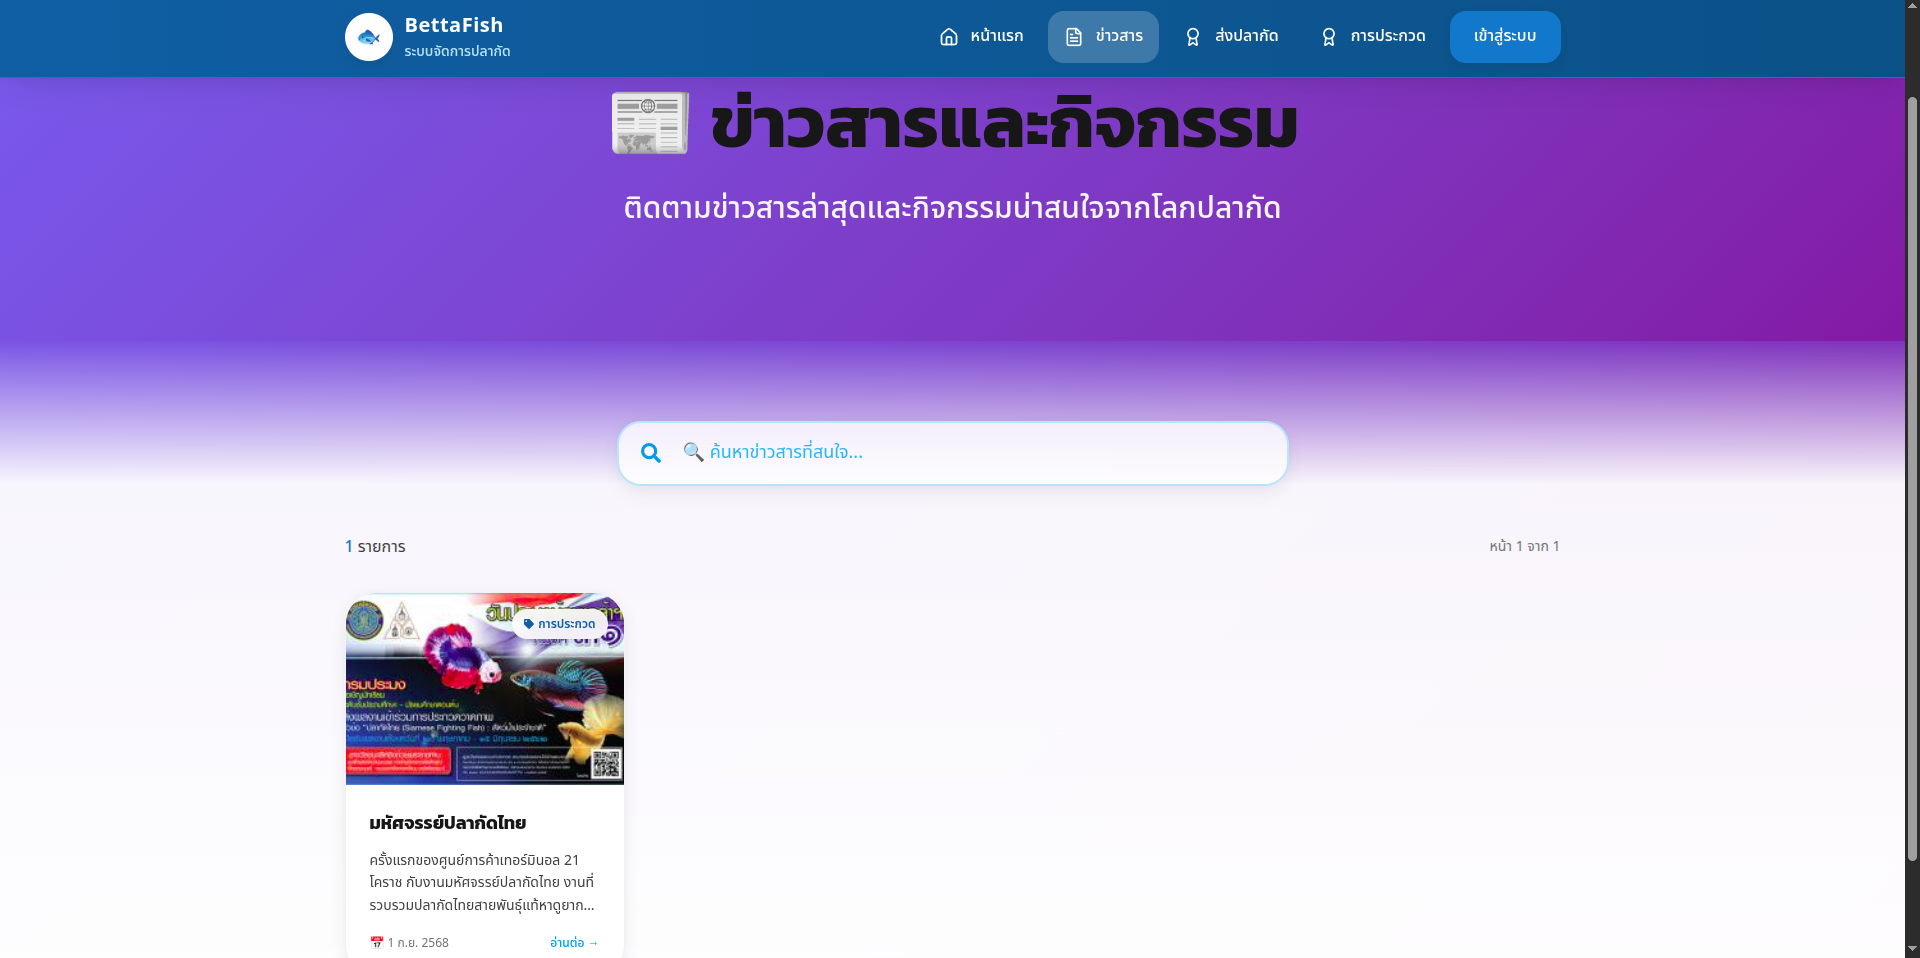
\includegraphics[width=0.8\linewidth]{HP2}
	\caption{หน้าข่าวสารทั้งหมดในระบบ}
\end{figure}

\indent ในหน้านี้ ผู้ใช้จะเจอกับรายการ "ข่าวสารและกิจกรรม" ทั้งหมดที่มีในระบบ โดยหลักๆ แล้ว ผู้ใช้จะสามารถ ค้นหาข่าวที่สนใจ ด้านบนสุดของหน้าจะมีช่องค้นหา ผู้ใช้สามารถพิมพ์คำค้นหาที่ต้องการลงไปได้เลยครับ เช่น ชื่อกิจกรรม หรือคำที่อยู่ในเนื้อหาข่าว ระบบก็จะกรองรายการข่าวที่เกี่ยวข้องมาให้ดูทันที
เลือกอ่านข่าวที่ต้องการ ข่าวแต่ละเรื่องจะแสดงเป็นการ์ดสวยงาม ผู้ใช้สามารถคลิกที่การ์ดข่าวเรื่องไหนก็ได้ที่สนใจ เพื่อเข้าไปอ่านรายละเอียดเนื้อหาทั้งหมดของข่าวนั้นๆ ในหน้าถัดไป
เลื่อนดูหน้าต่างๆ ถ้ามีข่าวเยอะมากๆ จนแสดงไม่หมดในหน้าเดียว ด้านล่างสุดจะมีปุ่มตัวเลขและปุ่ม "ก่อนหน้า" กับ "ถัดไป" ให้ผู้ใช้สามารถกดเพื่อเลื่อนไปดูข่าวในหน้าอื่นๆ ได้ครับ

\vspace{\baselineskip}

\begin{figure}[h]
	\centering
	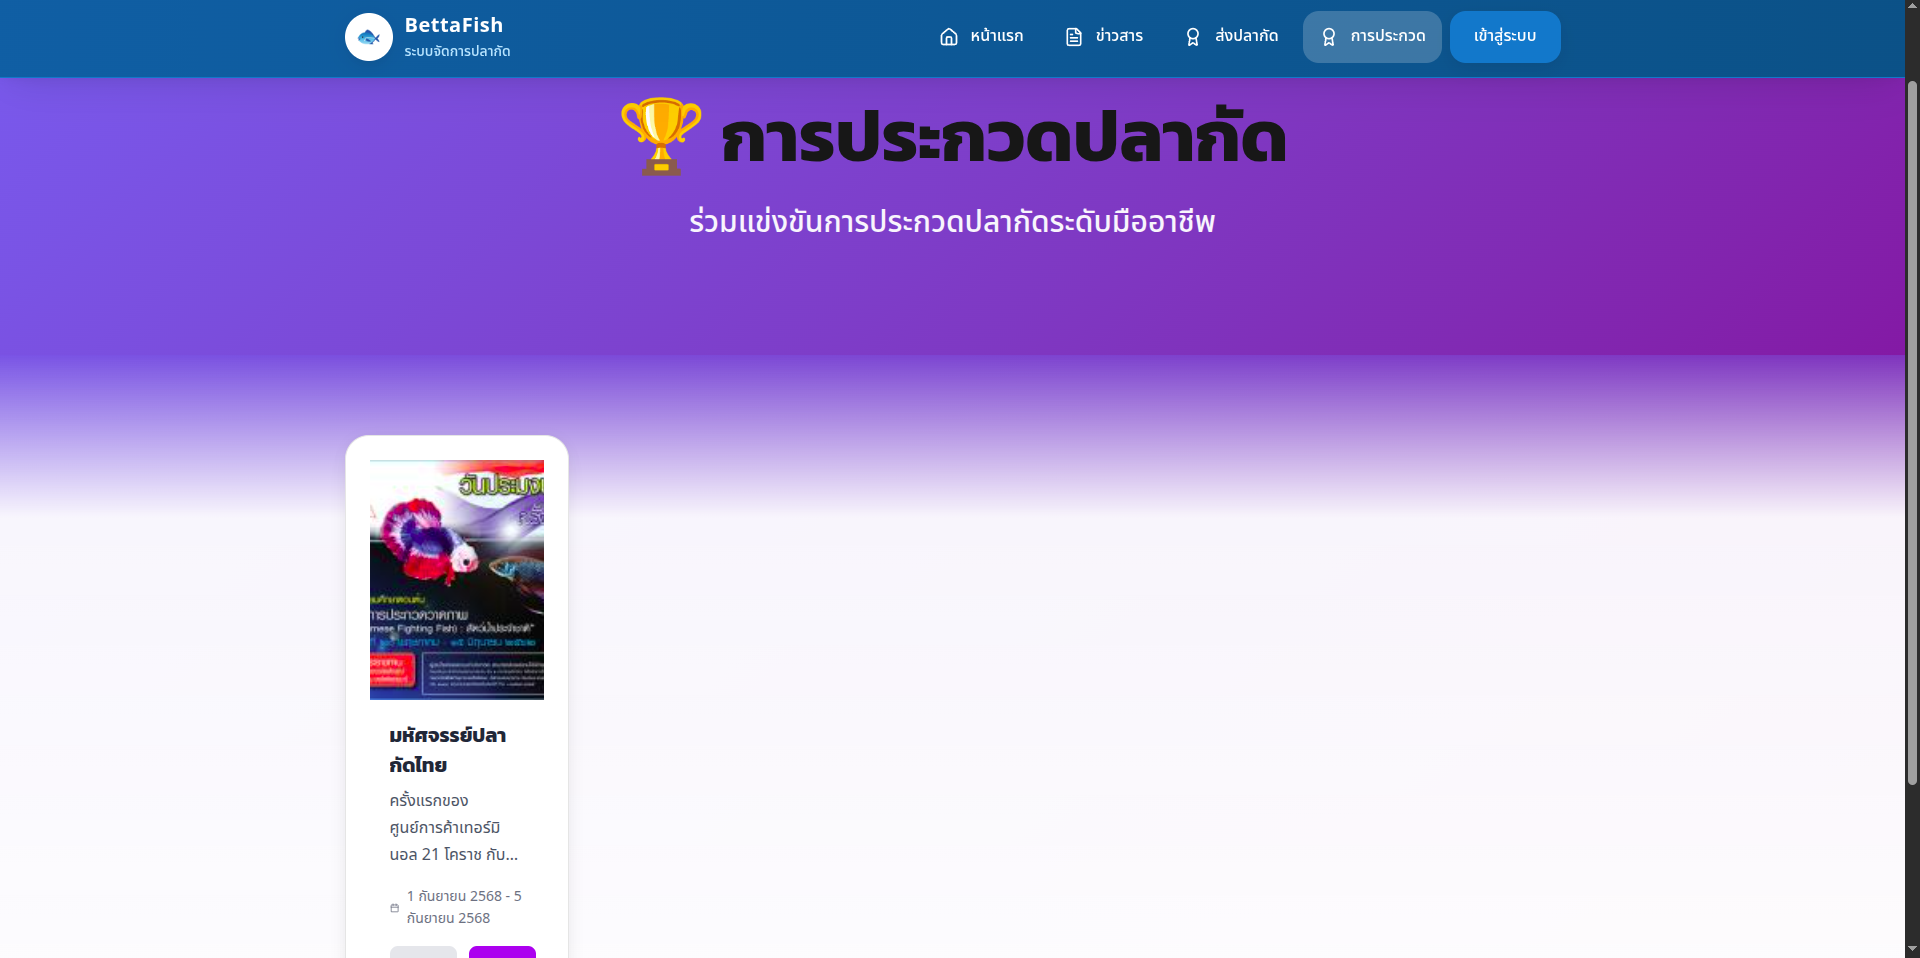
\includegraphics[width=0.8\linewidth]{HP3}
	\caption{หน้ารายการประกวด}
\end{figure}

\indent ในหน้าการประกวด จะแบ่งการใช้งานตามสถานะการล็อกอินของผู้ใช้ \textbf{ถ้ายังไม่ได้ล็อกอิน (ผู้ใช้ทั่วไป)} ดูได้ทุกอย่าง สามารถเข้ามาดูรายการประกวดทั้งหมดที่กำลังเปิดรับสมัครได้ เห็นโปสเตอร์กิจกรรม ชื่อกิจกรรม และรายละเอียดเบื้องต้นได้เหมือนกับคนที่ล็อกอินแล้วทุกอย่างเลย อ่านรายละเอียดได้ แต่จะยังเข้าร่วมไม่ได้ \textbf{ถ้าล็อกอินแล้ว (สมาชิก)} ดูได้ทุกอย่าง และสามารถเข้าร่วมประกวด

\newpage

\begin{figure}[h]
	\centering
	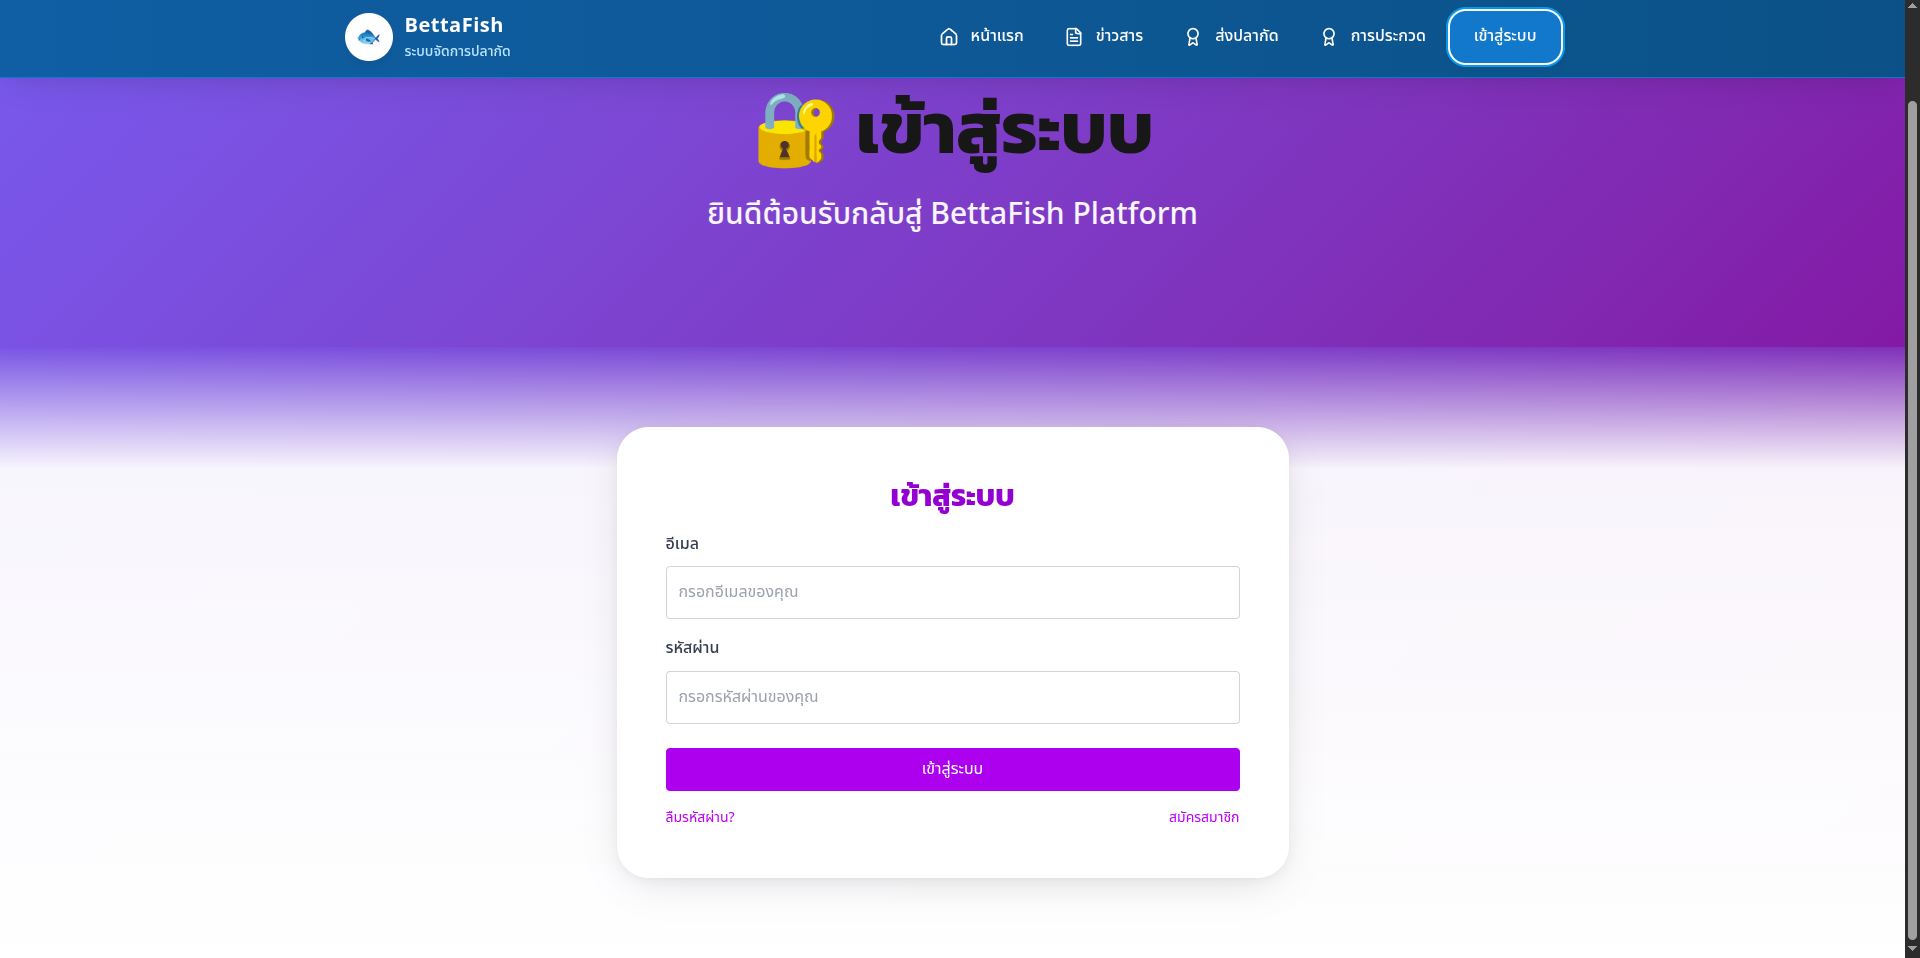
\includegraphics[width=0.8\linewidth]{LG1}
	\caption{หน้าเข้าสู่ระบบ}
\end{figure}

\indent ในหน้านี้ผู้ใช้สามารถเข้าสู่ระบบได้ และสามารถกดสมัครสมาชิกได้ กรณีไม่มีบัญชีเข้าใช้งาน

\vspace{\baselineskip}

\begin{figure}[h]
	\centering
	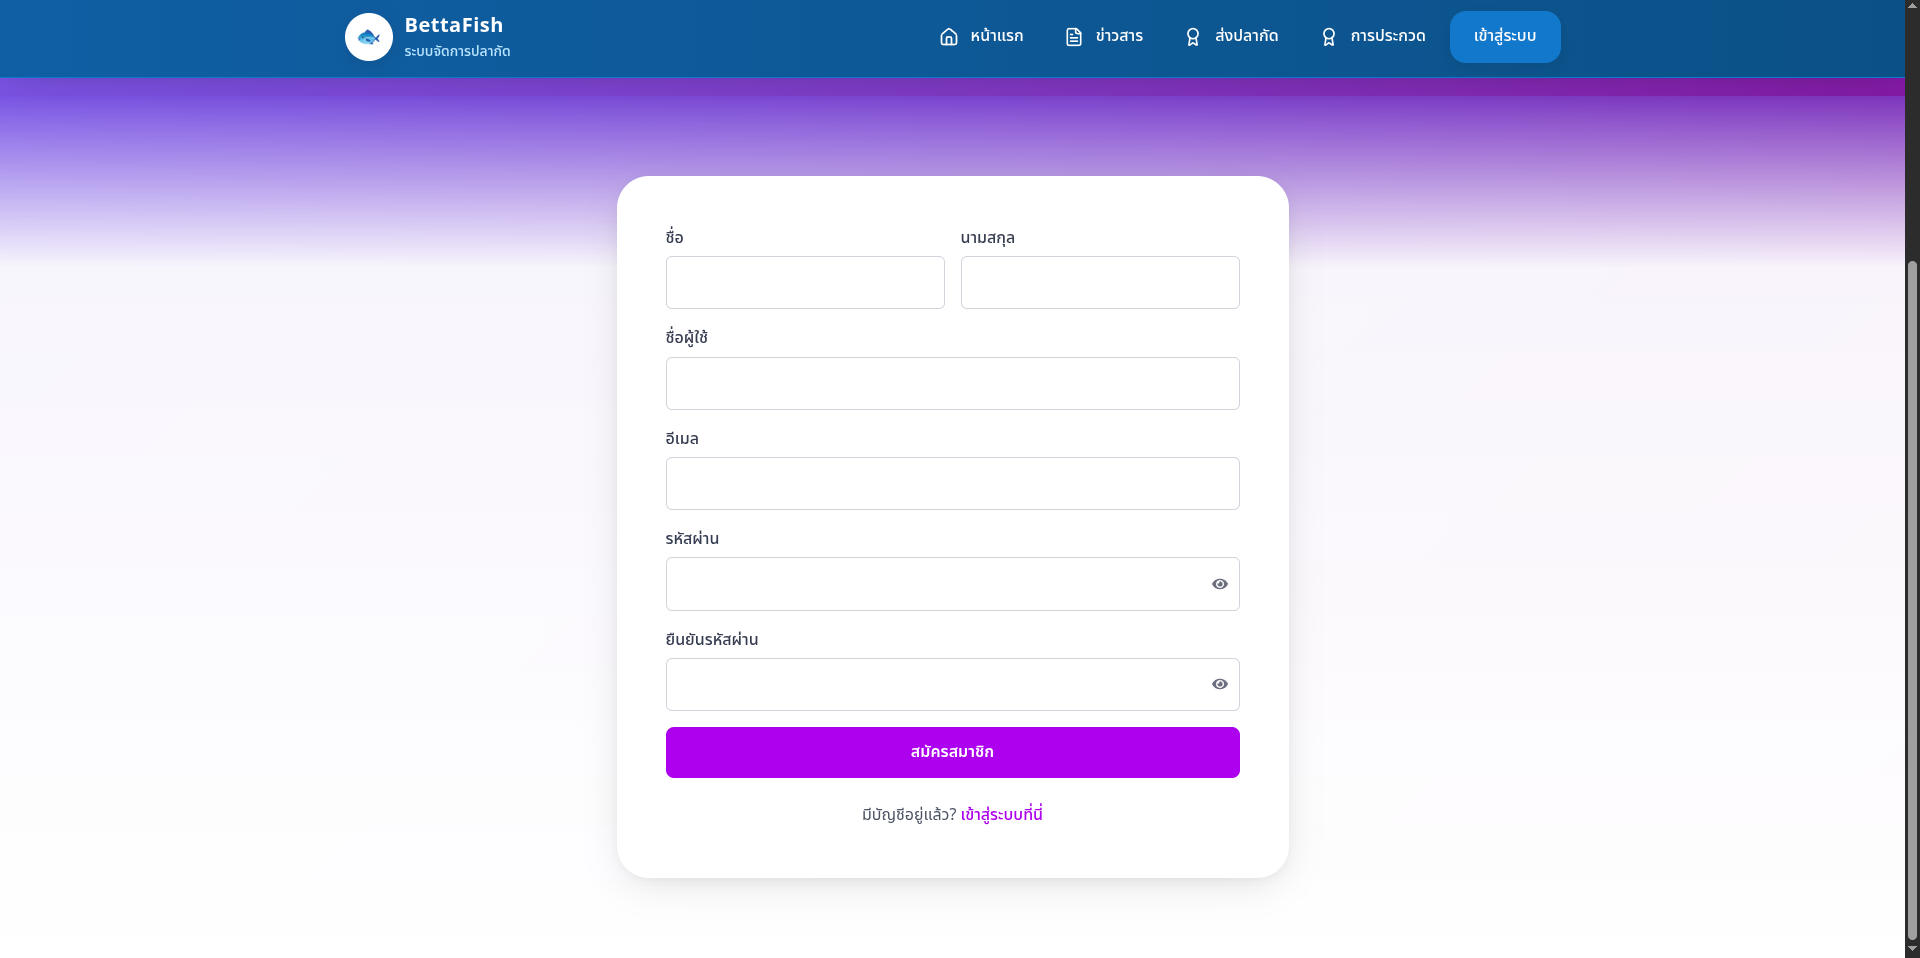
\includegraphics[width=0.8\linewidth]{RG1}
	\caption{หน้าสมัครสมาชิก}
\end{figure}

\indent ในหน้านี้ผู้ใช้สามารถสมัครสมาชิกได้โดยกรอกรายละเอียดตามแบบฟอร์มได้เลย

\newpage

\begin{figure}[h]
	\centering
	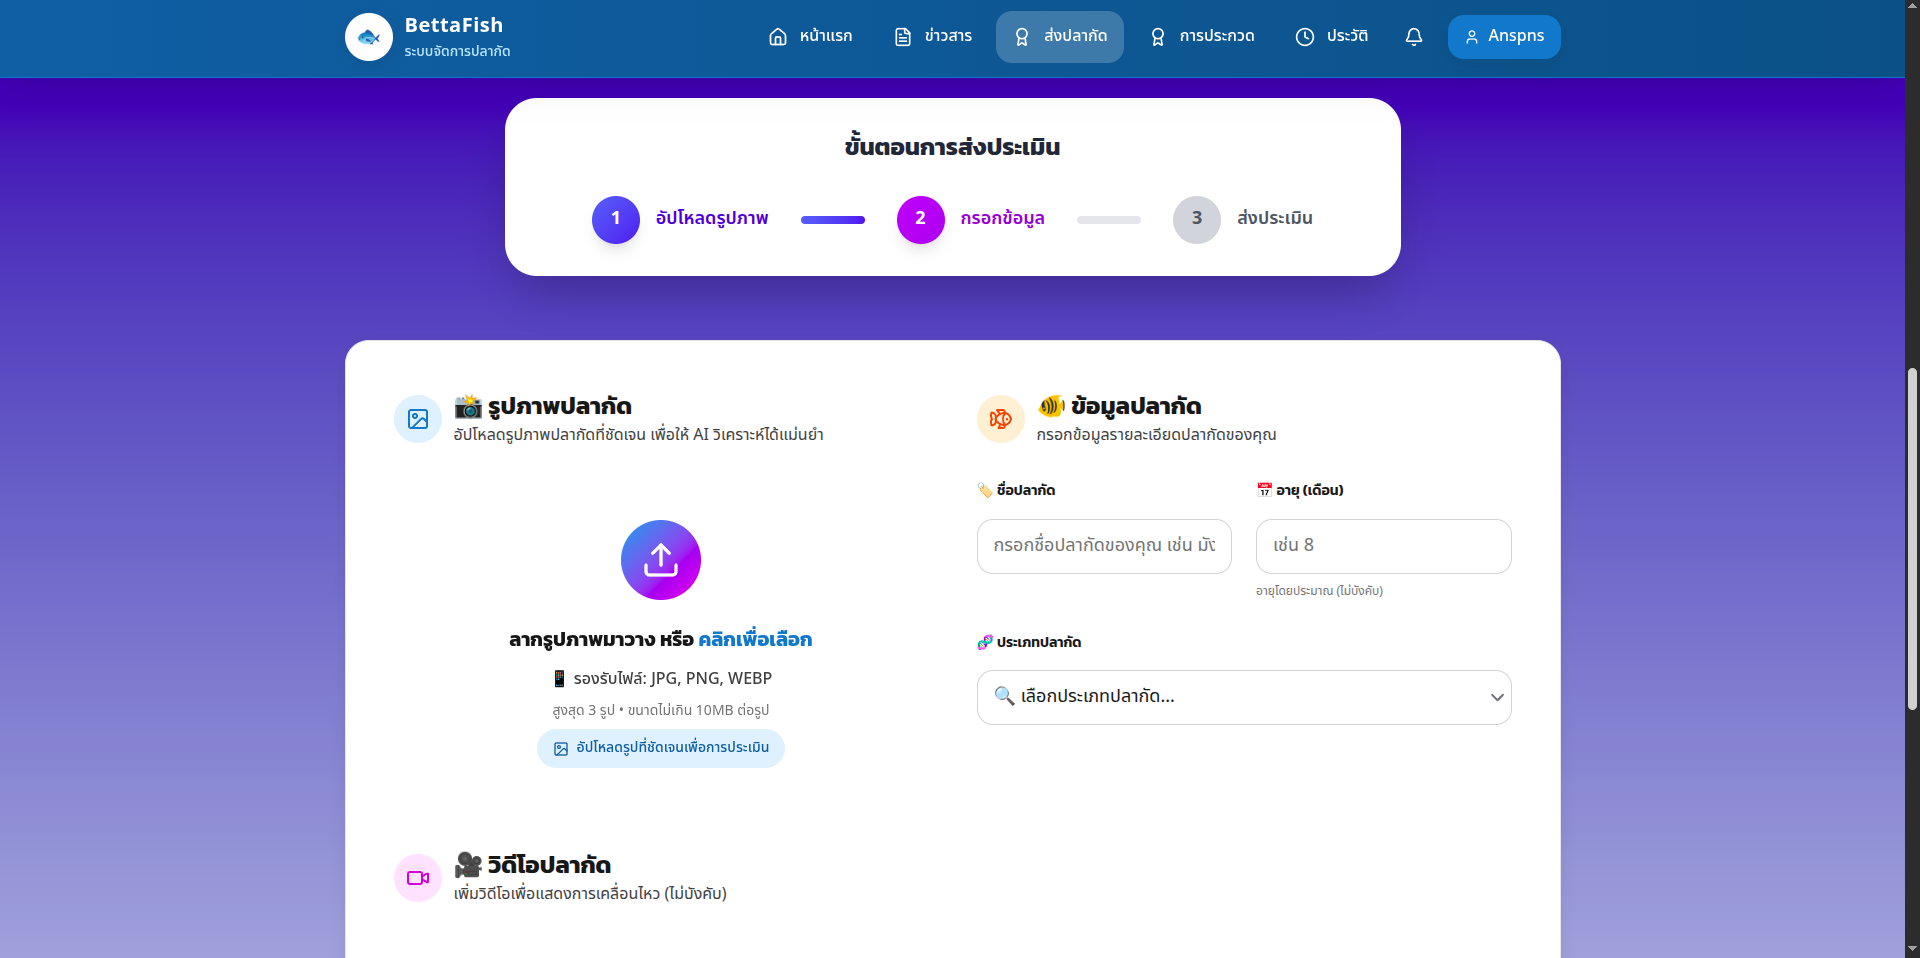
\includegraphics[width=0.8\linewidth]{EV1}
	\caption{หน้าประเมินคุณภาพปลากัด}
\end{figure}

\indent ในหน้านี้ผู้ใช้สามารถใส่ข้อมูลตามแบบฟอร์มได้เลย เช่นใส่รูปภาพ ใส่วิดีโอ ใส่ชื่อปลากัด ใส่ประเภทปลากัด เรามี Ai ช่วยตรวจสอบประเภทปลากัดตอนนี้เราสามารถทำได้ 3 ประเภท ได้แก่ ปลากัดพื้นบ้านมหาชัย ปลากัดพื้นบ้านภาคอีสานหางลาย และปลากัดพื้นบ้านภาคใต้

\vspace{\baselineskip}

\begin{figure}[h]
	\centering
	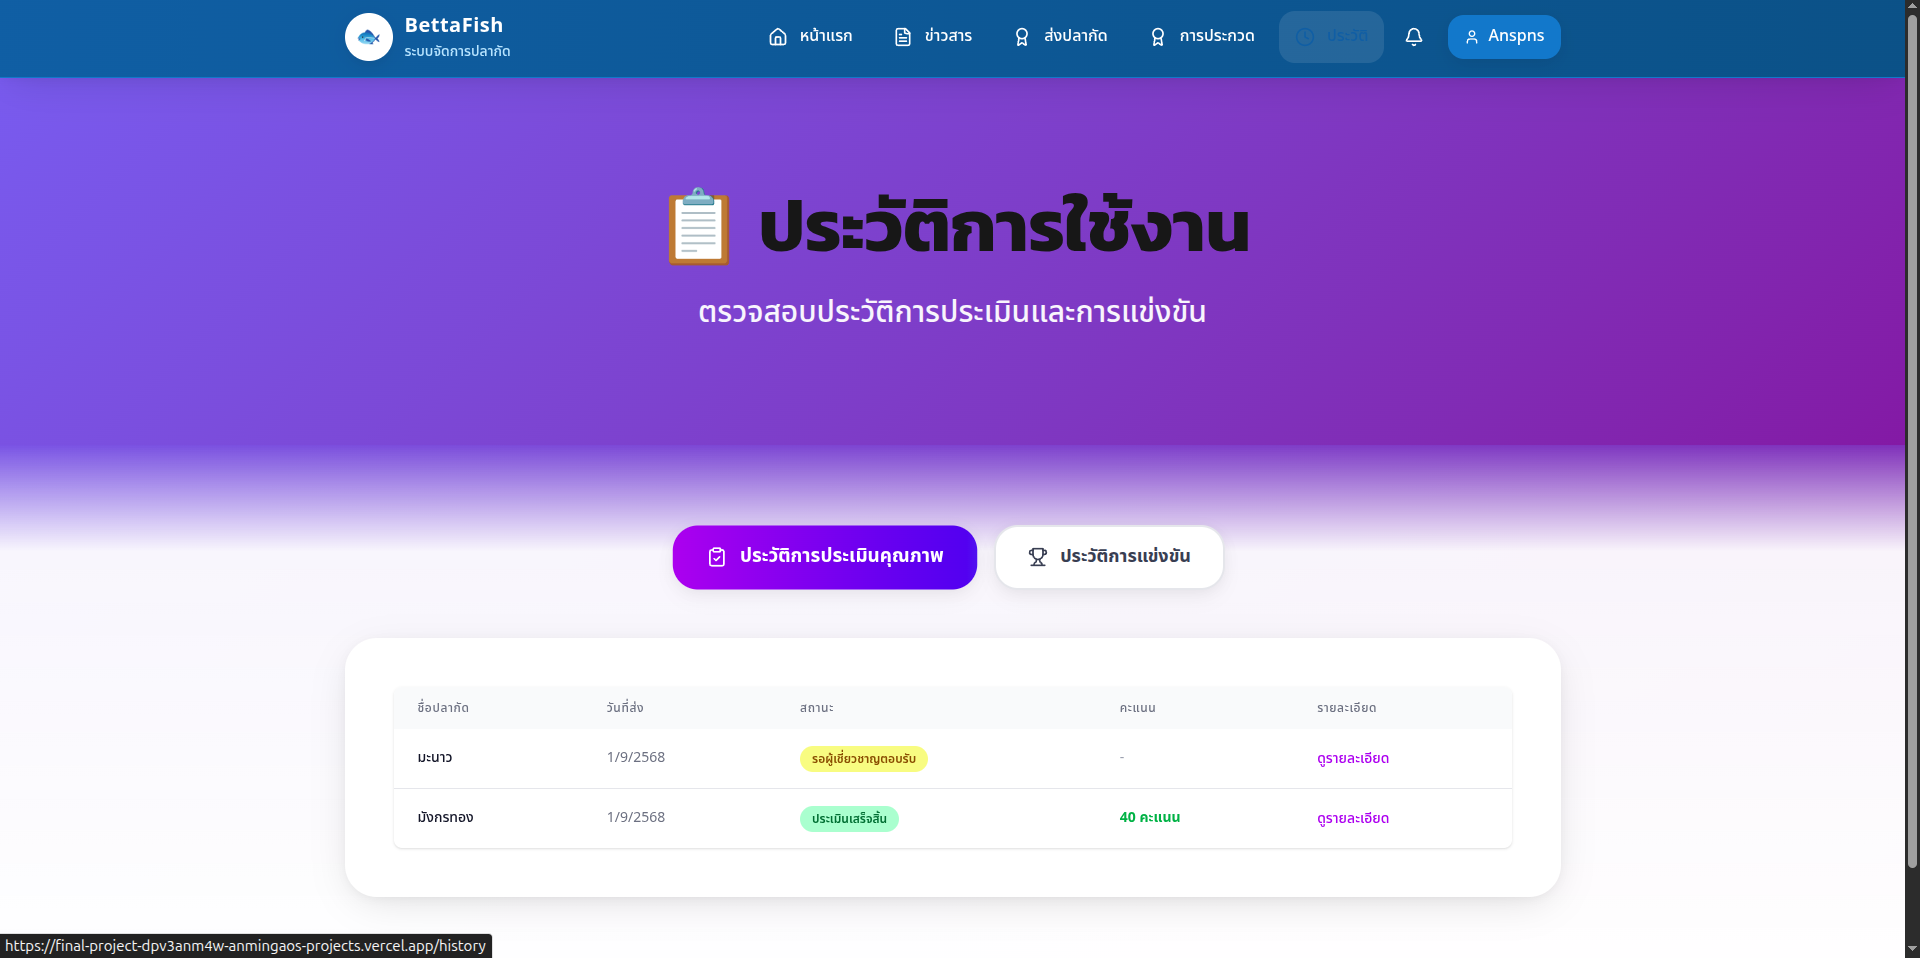
\includegraphics[width=0.8\linewidth]{HT1}
	\caption{หน้าประวัติการส่งประเมินคุณภาพปลากัด}
\end{figure}

\indent ในหน้านี้ผู้ใช้สามารถดูได้ว่าตนเองส่งปลากัดเข้าร่วมการประเมินคุณภาพไปกี่ครั้งแล้ว และสามารถดูคะแนนที่รับได้ 

\newpage

\begin{figure}[h]
	\centering
	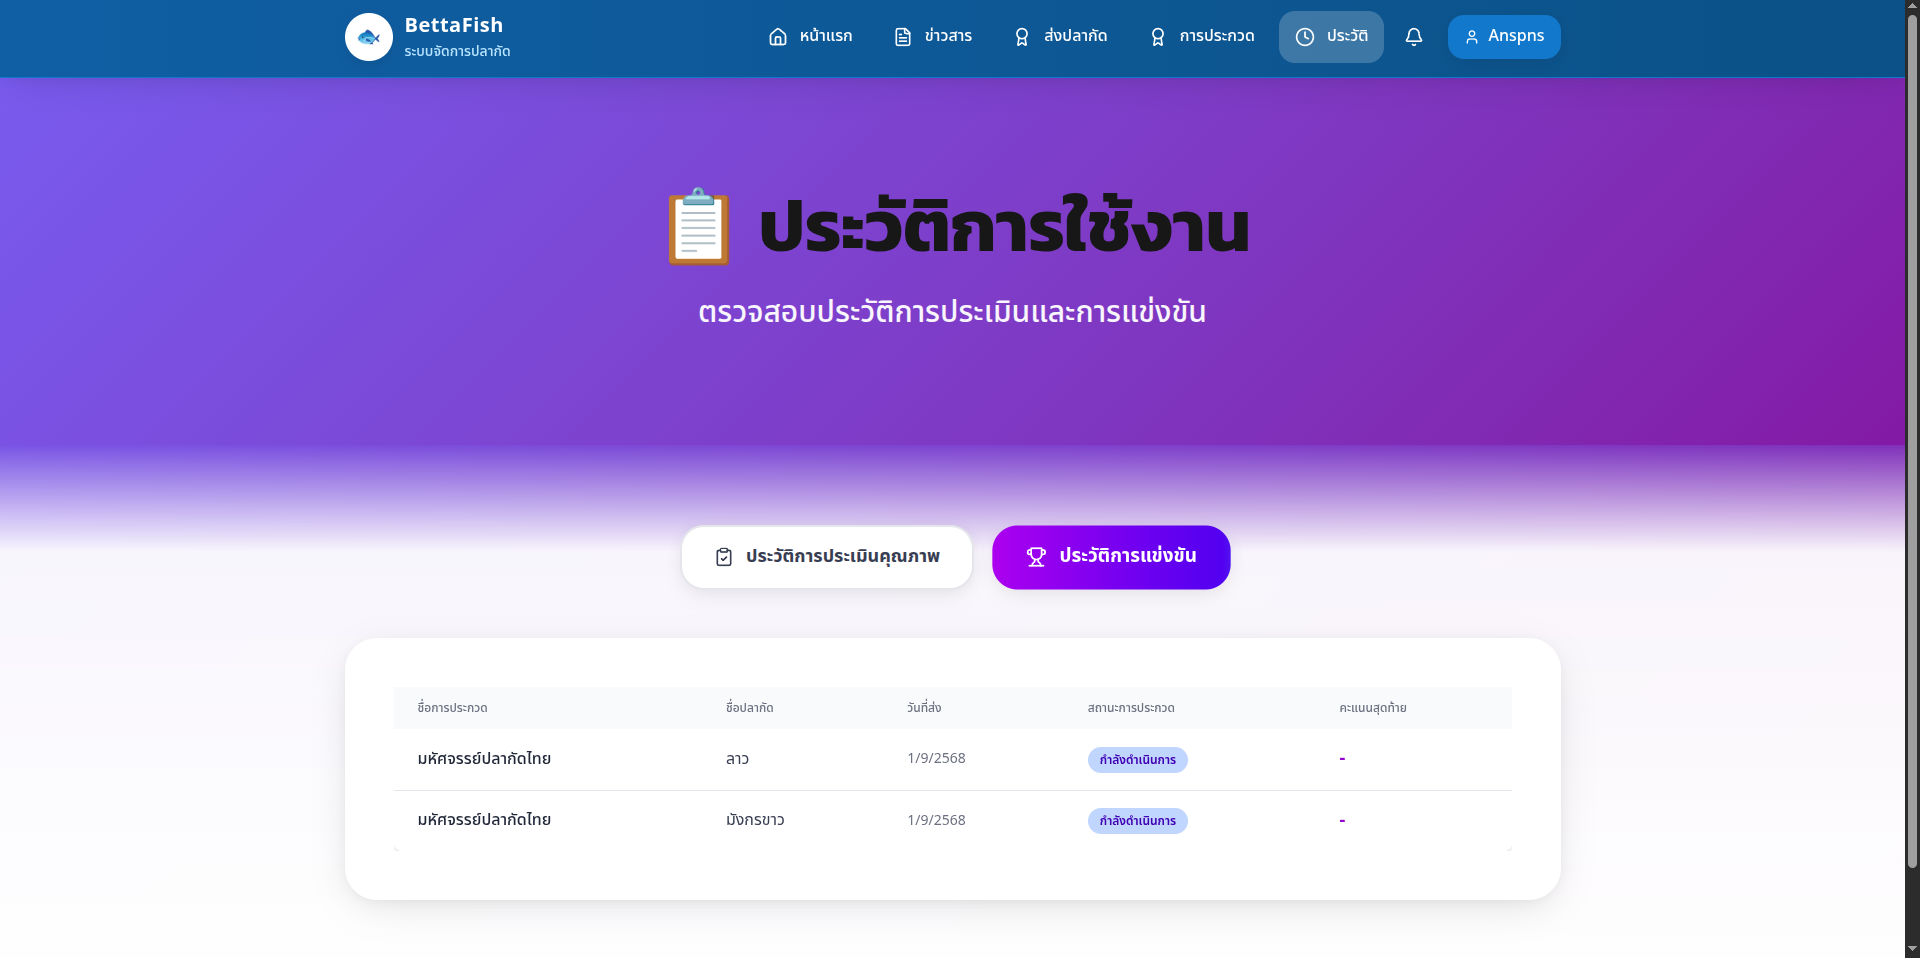
\includegraphics[width=0.8\linewidth]{HT2}
	\caption{หน้าประวัติการส่งประเมินคุณภาพปลากัด}
\end{figure}

\indent ในหน้านี้ผู้ใช้สามารถดูได้ว่าตนเองส่งปลากัดเข้าร่วมการประเกวดไปกี่ครั้งแล้ว และสามารถดูผลได้ว่าได้ลำดับที่เท่าไหร่

\vspace{\baselineskip}

\begin{figure}[h]
	\centering
	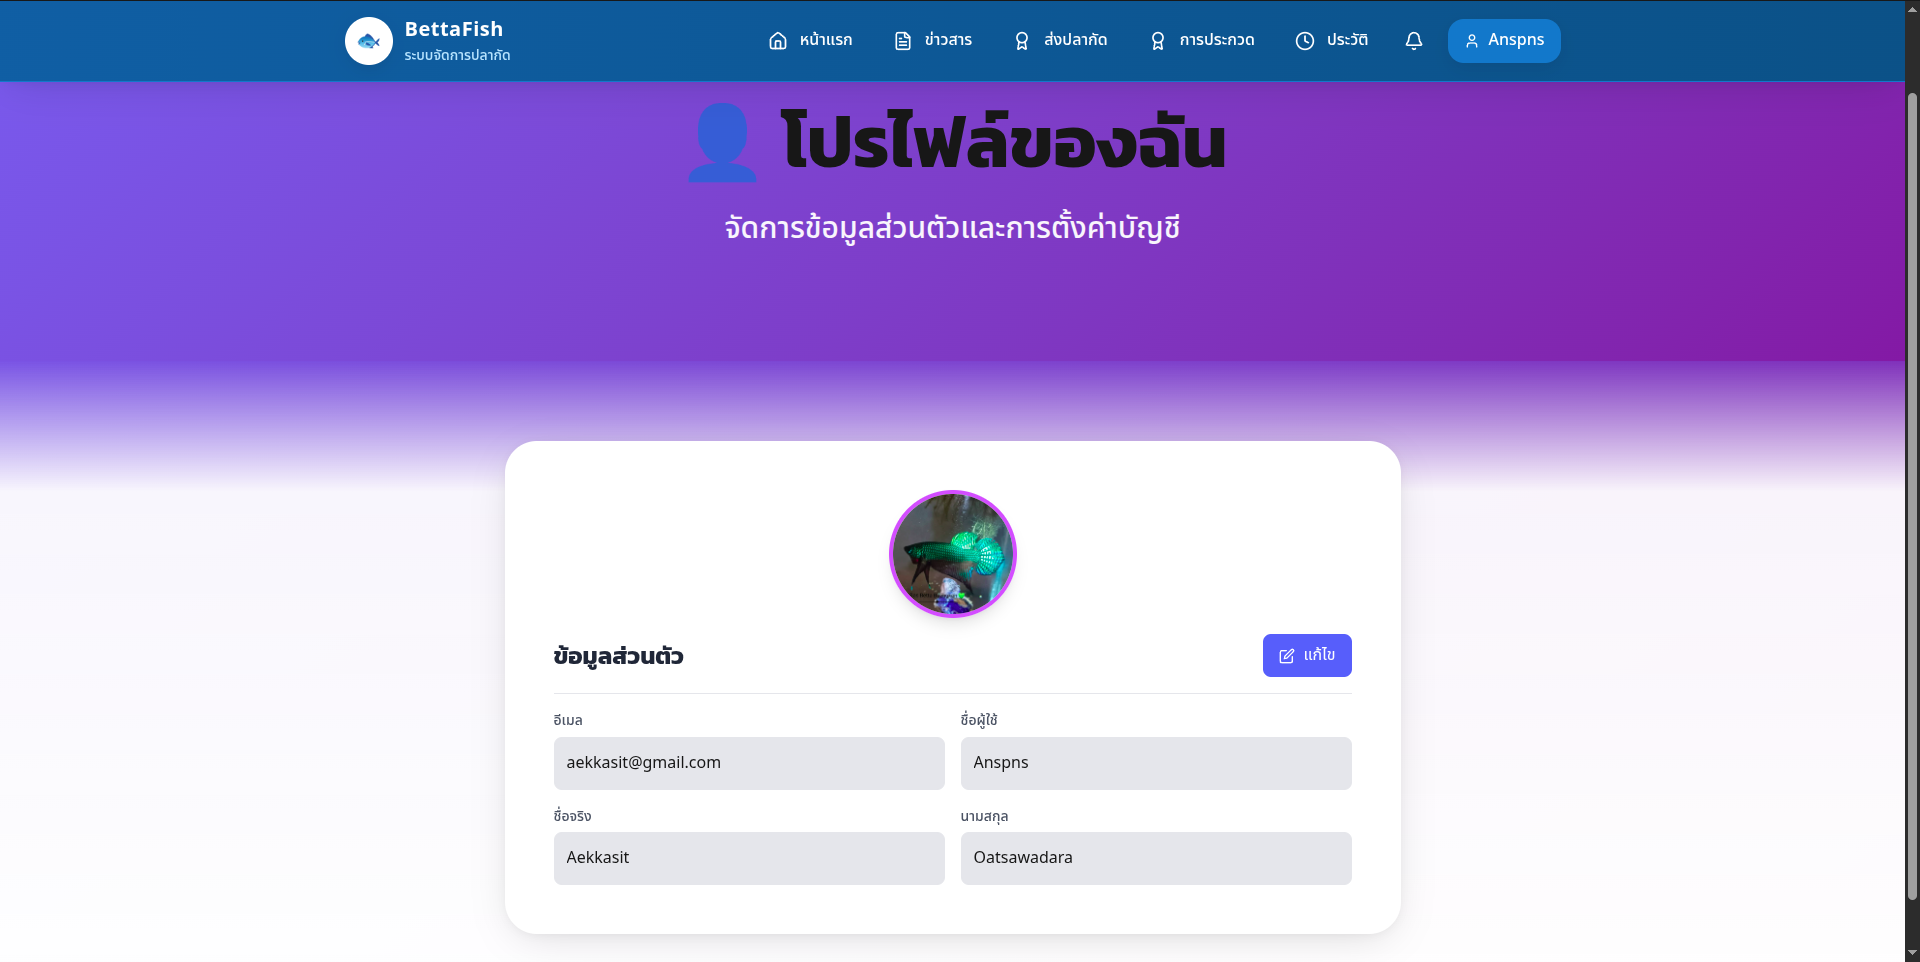
\includegraphics[width=0.8\linewidth]{PF1}
	\caption{หน้าโปรไฟล์ผู้ใช้}
\end{figure}

\indent ในหน้านี้ผู้ใช้สามารถแก้ไขข้อมูลส่วนตัวของตนเองได้และสามารถเปลี่ยบยนรูปภาพโปรไฟล์ได้

\newpage
	
	
\begin{sloppypar}
	\begin{enumerate}[start=2]  % เริ่มที่ 2 (ต่อจาก 1)
		\item \textbf{Web Application ผู้เชี่ยวชาญ}
	\end{enumerate}
\end{sloppypar}

\begin{figure}[h]
	\centering
	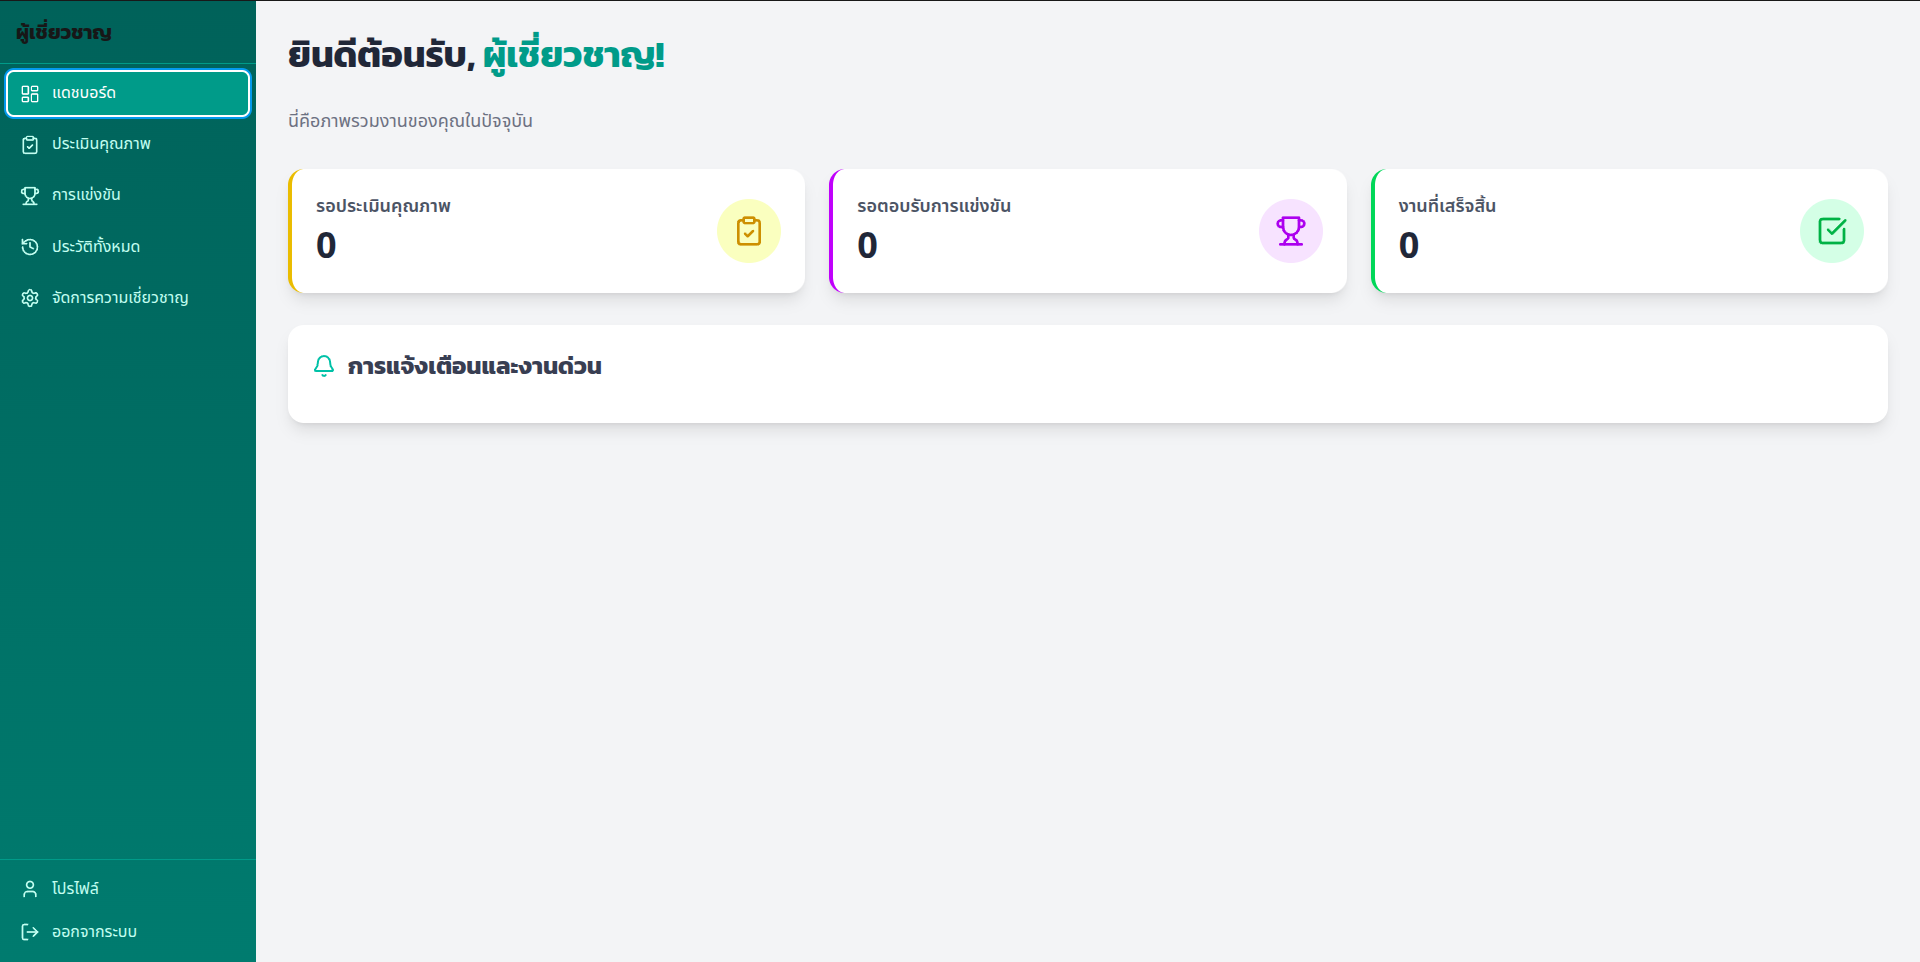
\includegraphics[width=0.8\linewidth]{EP1}
	\caption{หน้าหลักผู้เชี่ยวชาญ}
\end{figure}

\indent ในหน้านี้ ผู้เชี่ยวชาญสามารถ ดูภาพรวมของงานทั้งหมด ได้อย่างรวดเร็วผ่านการ์ดสรุป 3 อันหลักๆ คือ 
"รอประเมินคุณภาพ" บอกจำนวนปลากัดที่ถูกส่งมาให้ประเมินและกำลังรอให้เราจัดการ
"รอตอบรับการแข่งขัน" บอกจำนวนการแข่งขันที่ผู้จัดการ (Manager) ได้ส่งคำเชิญมาให้เราเป็นกรรมการ
"งานที่เสร็จสิ้น" สรุปจำนวนงานทั้งหมดที่เราได้ประเมินหรือตัดสินไปแล้ว 

\vspace{\baselineskip}

\begin{figure}[h]
	\centering
	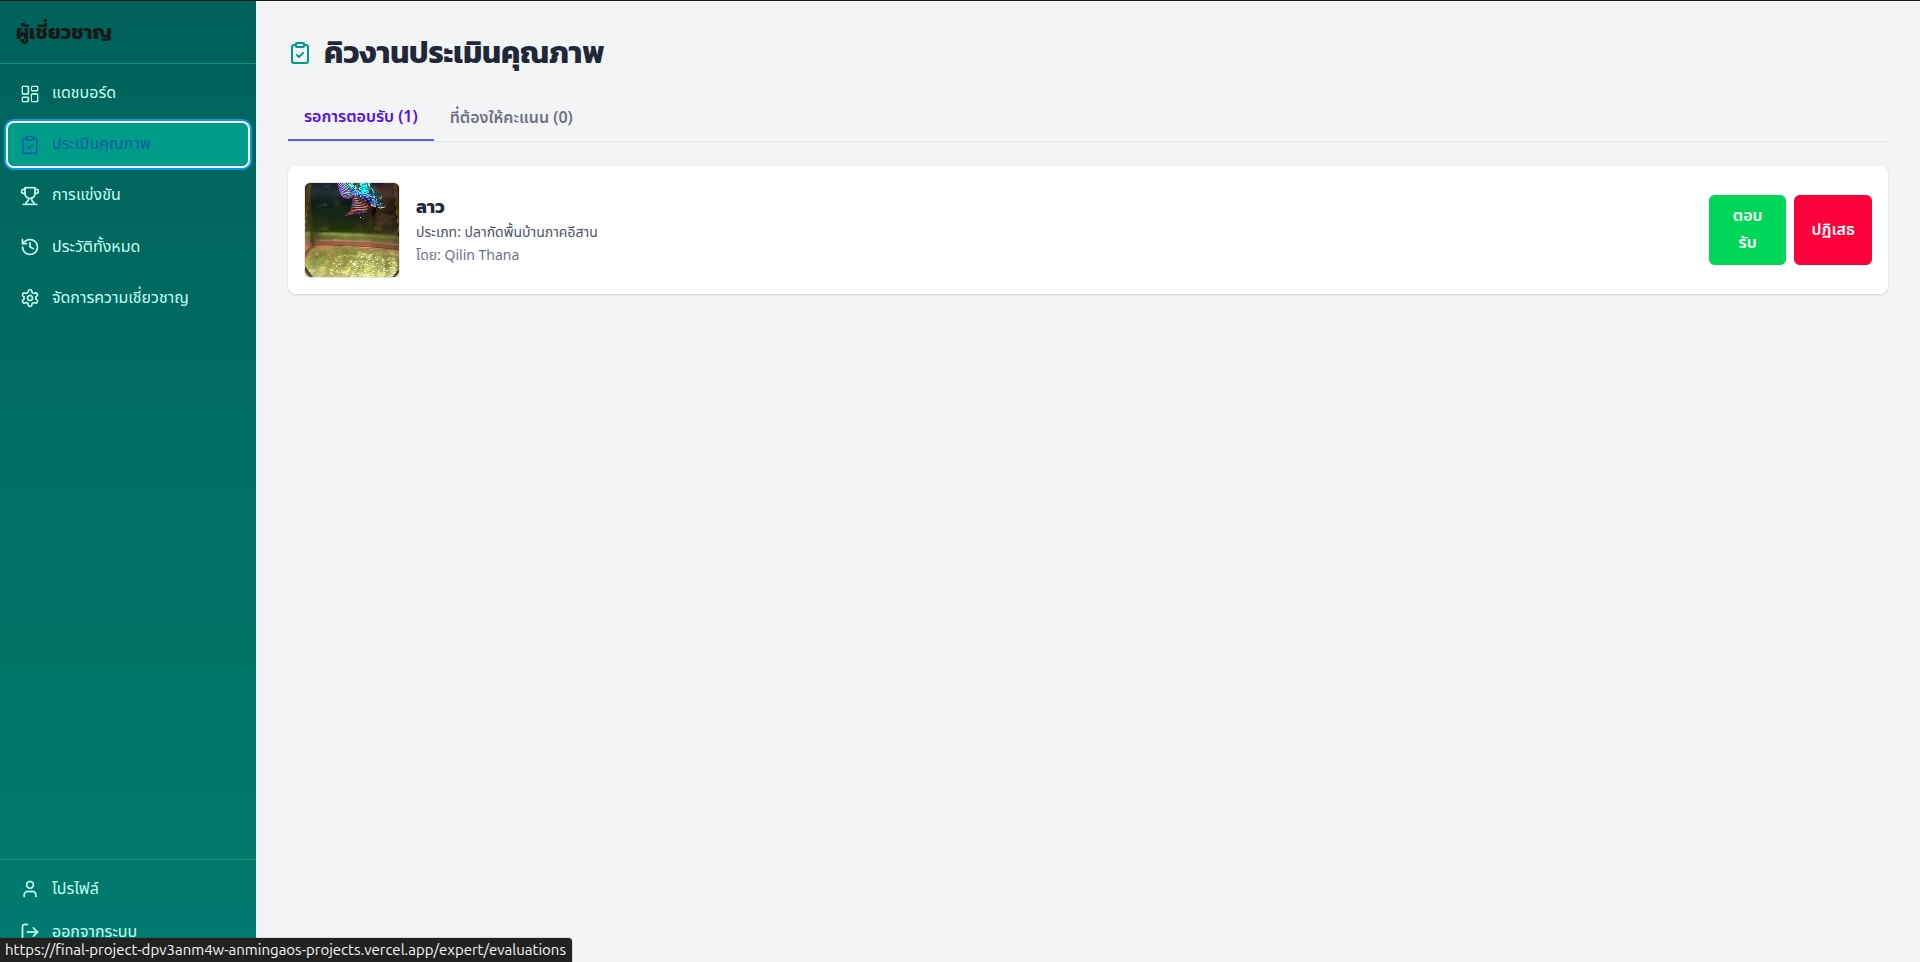
\includegraphics[width=0.8\linewidth]{EP2}
	\caption{หน้าคิวงานผู้เชี่ยวชาญ}
\end{figure}

\indent ในหน้านี้ ผู้เชี่ยวชาญสามารถดูงานที่ได้รับมอบหมาย ผู้เชี่ยวชาญจะเห็นรายการปลากัดที่ระบบมอบหมายมาให้ พร้อมข้อมูลเบื้องต้นอย่างรูปภาพ, ชื่อ, และประเภทของปลา ตัดสินใจรับงาน ผู้เชี่ยวชาญมี 2 ตัวเลือก กดปุ่ม "ตอบรับ" (สีเขียว) เพื่อยืนยันว่าจะทำงานประเมินชิ้นนี้ เมื่องานถูกตอบรับแล้ว ก็จะย้ายไปอยู่ในแท็บ "ที่ต้องให้คะแนน"
กดปุ่ม "ปฏิเสธ" (สีแดง) ในกรณีที่ไม่สะดวกประเมิน หรือเห็นว่าข้อมูลที่ส่งมาไม่เหมาะสม ก็สามารถปฏิเสธงานชิ้นนี้ได้

\endgroup